\section {Background}

\subsection {Bonding Coordination}

A hydrated \suldiox~in an aqueous environment forms hydrogen bonds through the oxygens to nearby water hydrogens, or interacts via the sulfur atoms with water oxygens. To further our analysis of the way in which \suldiox~coordinates its bonding to surface waters, we adopt a naming scheme to denote the way in which the \suldiox~is hydrated by the surrounding waters. This naming scheme mimics a notational system developed during a previous study on water coordination by Buch et al,\cite{Buch 2005} and was subsequently used in other computational work.\cite{Walker2006b} In this naming system, a letter is used to designate the atom on a water molecule through which a hydrogen bond is formed to neighboring waters. Thus a bonding coordination of ``OOH'' designates two proton-accepting bonding interactions through the water oxygen, and a single proton-donor bonding interaction through a hydrogen. More recently, Baer et al devised a nomenclature that explicitly enumerates the bonding to \suldiox~via the sulfur or oxygen atoms.\cite{Baer2010} 

In this work we port Buch et al's nomenclature to \suldiox~in order to show the amount of hydrogen bonding through the acceptor \suldiox-oxygens, and the weaker bonding interactions form from the \suldiox-sulfur to water oxygens. Thus, an ``SOO'' coordinated \suldiox~molecule forms a single interaction through the sulfur atom to a neighboring water oxygen, and two hydrogen bonds through either a single \suldiox-oxygen, or distributed with one hydrogen bond on each of the \suldiox~oxygens. Analysis of the distribution of \suldiox~coordinations will give insight to how it binds to the water surface.

During the course of the analysis we use the definition of bonds of Baer et al. in determining the \suldiox~bonding coordinations.\cite{Baer2010} The definition is formed from a set of distance criteria where a bonding interaction between a \wat-oxygen and \suldiox-sulfur is formed at a distance less than 3.5 \angs, and an \suldiox~oxygen hydrogen bond to a \wat-hydrogen is formed at a distance less than 2.2 \angs.

\subsection {Cyclic Bonding Structures}

Hydrated \suldiox~clusters have been studied extensively with many recent experiments and computations congealing to a clearer picture of \suldiox~bulk and surface behaviors.\cite{Baer2010, Tarbuck2005, Tarbuck2006, Ota2011, Bishenden1998, Hirabayashi2006, Steudel2009, Yang2002, Hayashi1985, Moin2011, Eckl2008} At a water surface, it is now known that \suldiox~forms a complex with water during adsorption, and then subsequently absorbs into the interfacial region by reaction to form ionic sulfur species.\cite{Tarbuck2005, Tarbuck2006, Ota2011} The first attempt to elucidate the structure of the surface hydrated \suldiox~by Baer et al. showed that the bonding coordination distributions of \suldiox~at the surface are altered relative to the bulk region, and that two coordinations dominate the distribution of bonding types: the ``SO'' and the ``SOO''. In the same work they then focused on the most dominant coordination to determine the most likely cluster geometry using two and three-water clusters bound to the \suldiox.

The cluster geometries found in Baer's study of the surface \suldiox~hydrates imply a cyclic bonding structure through the two or three waters involved. This is manifested as a closed loop formed by the intermolecular hydrogen bonds, S-O interactions, and covalent bonds of the molecules involved. Figure \ref{fig:cyclic-example} depicts one such cyclic structure showing the bonds beginning on the \suldiox-sulfur and returning through the \suldiox-oxygen in a two-water cluster.

\begin{figure}[h!]
	\begin{center}
		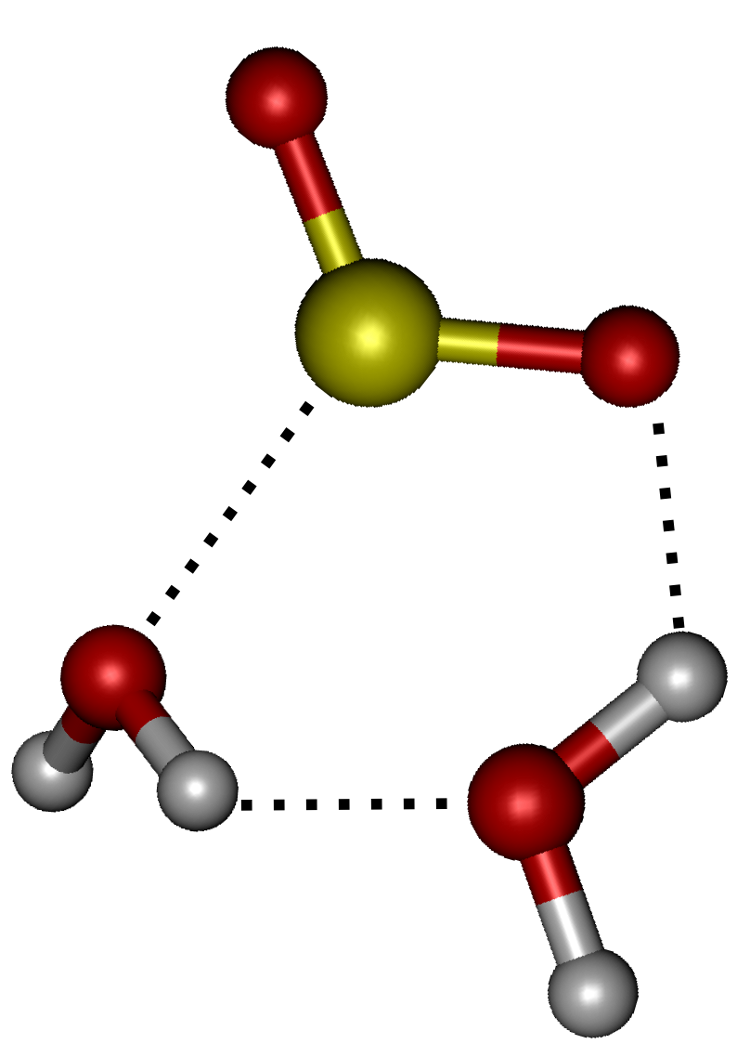
\includegraphics[scale=1.0]{images/cycles/double-cycle-type2-small.png}
		\caption{}
		\label{fig:cyclic-example}
	\end{center}
\end{figure}

The optimized geometry of the \suldiox-hydrates suggest cyclic bonding structures, but it remains a different story entirely when a \suldiox~is placed in a dynamic environment such as in the course of molecular dynamics simulations of an aqueous surface. Although geometry optimization shows the formation of these cyclic complexes, do they form during a dynamic bonding process on a simulated water surface? Graph theoretical techniques can be employed to determine if cyclic structures form during the simulations. Previous use of graphs in molecular computations were applied to finding stable arrangements of water clusters, ice, hydrogen bonding, extracting topological molecular properties, and cyclic structure studies.\cite{Anick2002, Huber2007, Radhakrishnan1991, Shi2005, Garcia2004, McDonald1998}

Here we will only briefly introduce graph theoretical concepts as they have been described well by others, and with varied application to cyclic structures.\cite{Tutte1984, Balakrishnan2000, Harary1973, Huber2007, Garcia2004, Dury2001} A graph consists of a set of vertexes, and edges that connect the vertexes. A molecule can be represented with atoms as vertexes, and edges for each intramolecular covalent bond connecting the atoms. The set of edges is then further expanded to include intermolecular interactions such as hydrogen bonds and other bonding bonding interactions. Edges may be assigned weights (i.e. bond lengths), types, and can be directional pointing towards a specific target from a source. A molecular system including all atoms, bonds, and interactions is thus fully described by a graph. 

To detect cyclic structures in a graph a depth-first or breadth-first search (DFS and BFS, respectively) may be used.\cite{Knuth1997, Cormen 2001} A BFS is a recursive algorithm of queuing vertexes and all adjacent neighboring vertexes while performing a specified procedure on each visited vertex. This is easily performed on adjacency list or connectivity matrix data structures, iterating through atoms of interest in the graph as starting points of the search. In BFS terminology, all nodes are colored during graph traversal to distinguish unvisited nodes (white), queued nodes (gray), and visited nodes (black). Using a BFS on a graph, cyclic structures are detected any time a ``gray target'' is encountered when queuing adjacent neighbors of a vertex. A benefit of BFS on a graph is the ability to determine the smallest cyclic structure in which a given vertex is a member. In the case of \suldiox~hydrate structures, beginning the BFS with the \suldiox~sulfur as the root vertex will discover cyclic bonding structures in order of size. Here we are only concerned with the smallest cyclic structure involving those waters in the first and second hydration shells around the \suldiox. Furthermore, it is possible to reconstruct a cycle's structure to find the size of the cycle (number of atoms involved), the number of unique waters in the cycle, and the type of cyclic structure encountered.

The various types of cyclic bonding arrangements are shown in Figure \ref{fig:cyclic-structures} for a \suldiox~molecule bonding to waters. Although three waters are shown in the molecular cartoon, any number of waters are allowed. Also, further bonding may occur to any of the participating molecules extraneous to the cyclic structure. Cycle types \Rmnum{1}, \Rmnum{2}, \Rmnum{3} in Figure \ref{fig:cyclic-structures} are cyclic structures in which the \suldiox~is a member of the cycle. Types \Rmnum{4} and \Rmnum{5} do not involve the \suldiox~in the bonding cycle, but are commonly encountered as the smallest cycle formed near the \suldiox. Type \Rmnum{3} is of particular interest because it is one of the most dominant \suldiox~bonding coordinations (``SO'', as shown later) configured as a cyclic structure. 

\begin{figure}[h!]
	\begin{center}
		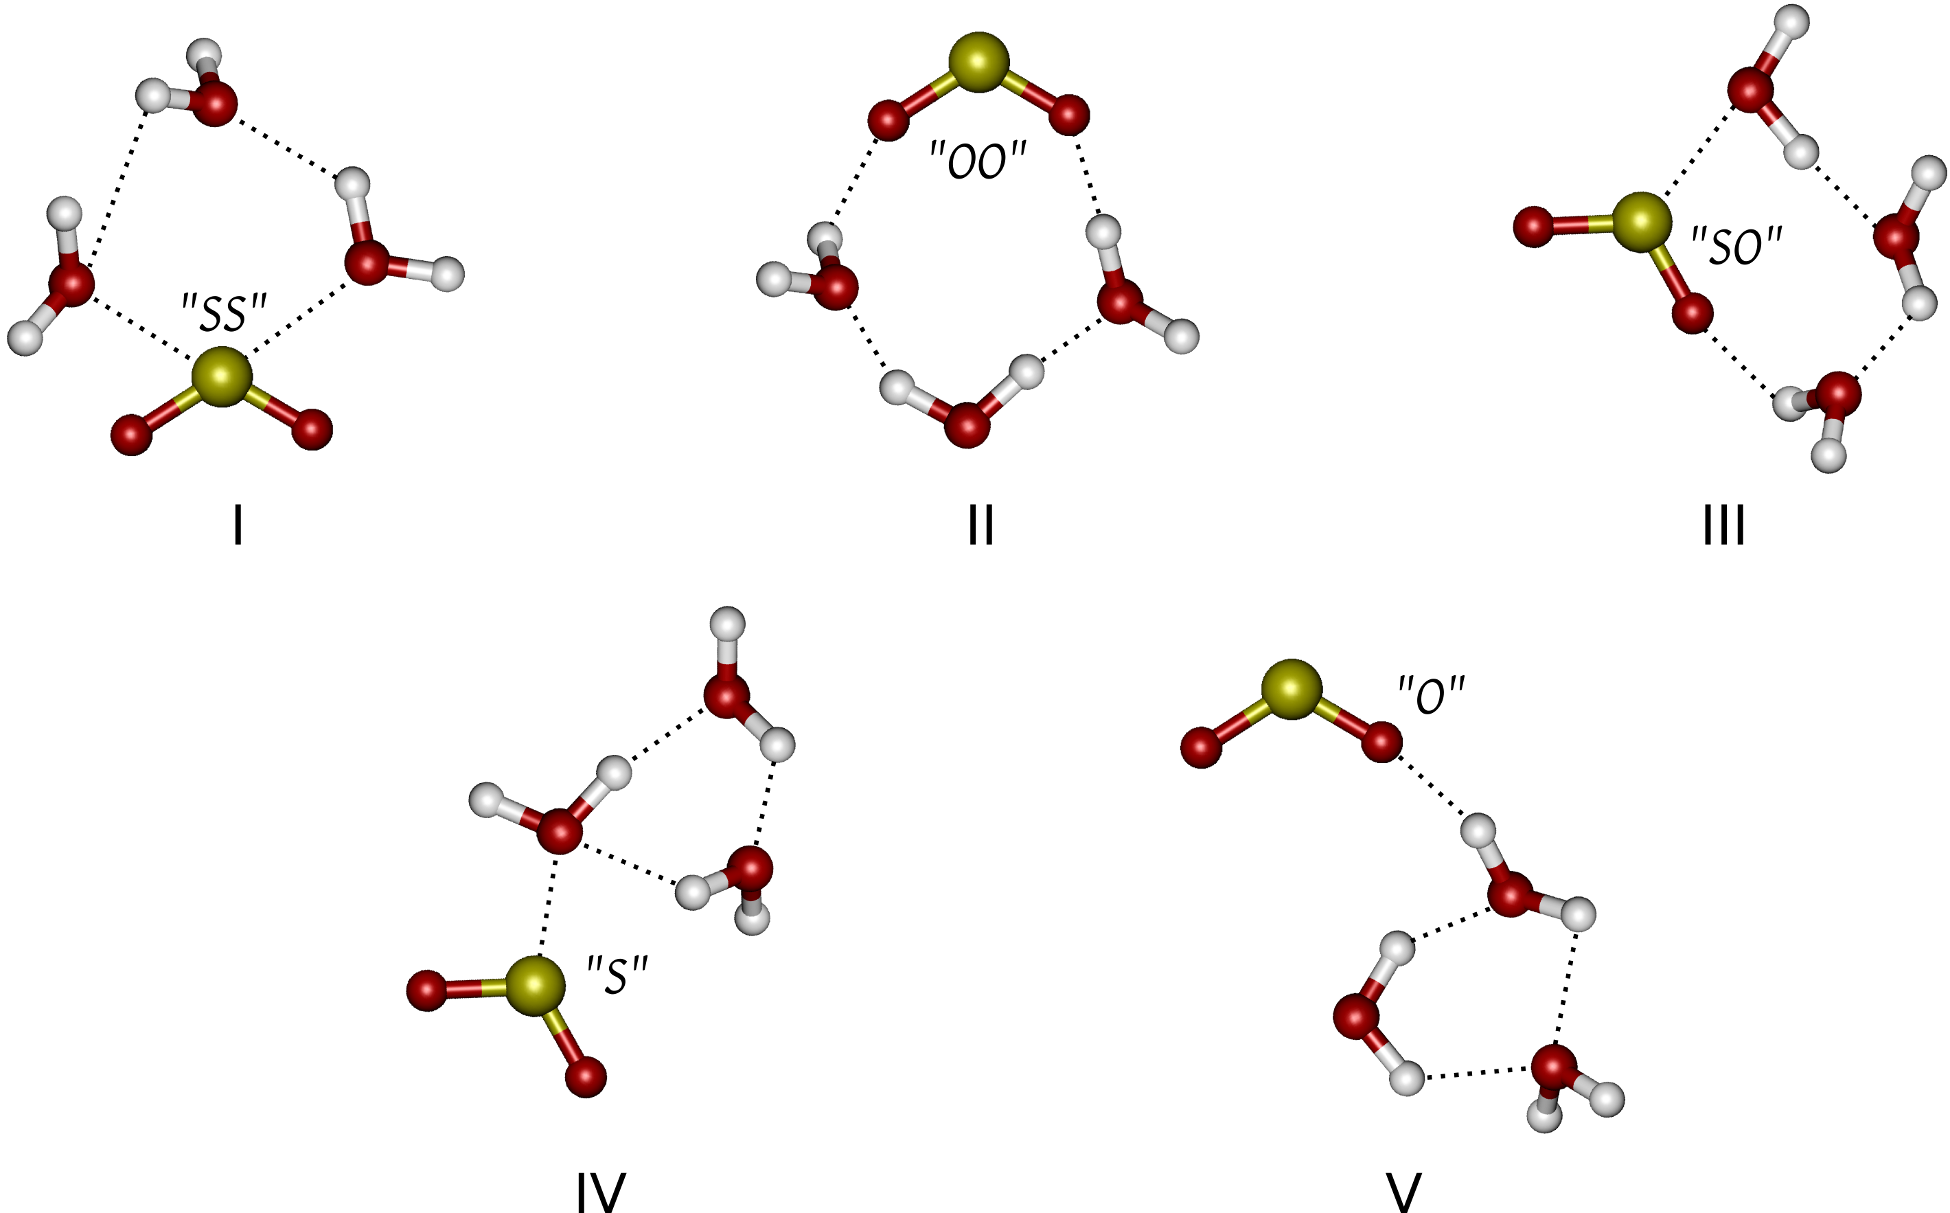
\includegraphics[scale=1.0]{images/cycles/cycle-types-small.png}
		\caption{}
		\label{fig:cyclic-structures}
	\end{center}
\end{figure}

Baer et al. presented a detailed geometric and spectroscopic breakdown of type \Rmnum{3} cycles with two and three waters from their DFT calculations.\cite{Baer2010} Given the information of the number of waters, atoms, and bonds involved in the bonding cycles, we find that of the three-water type \Rmnum{3} cycles, there exist two structural varieties, shown in Figure \ref{fig:type-3-varieties}, that differ in the arrangement of the waters involved. Type \Rmnum{3}-A (shown in Figure \ref{fig:type-3-varieties}A) is arranged with each water contributing an OH bond to the structure of the cycle. Type \Rmnum{3}B involves a single water contributing an OH, whereas the other two waters contribute only the oxygen atom or the entire water molecule to the structure, respectively. This nuance of the three-water type \Rmnum{3} structures, and the overall distribution are presented in more detail later. We also show the distribution of cyclic structures encountered during MD simulations to further understand the behaviors of \suldiox-hydrates at the water surface.

\begin{figure}[h!]
	\begin{center}
		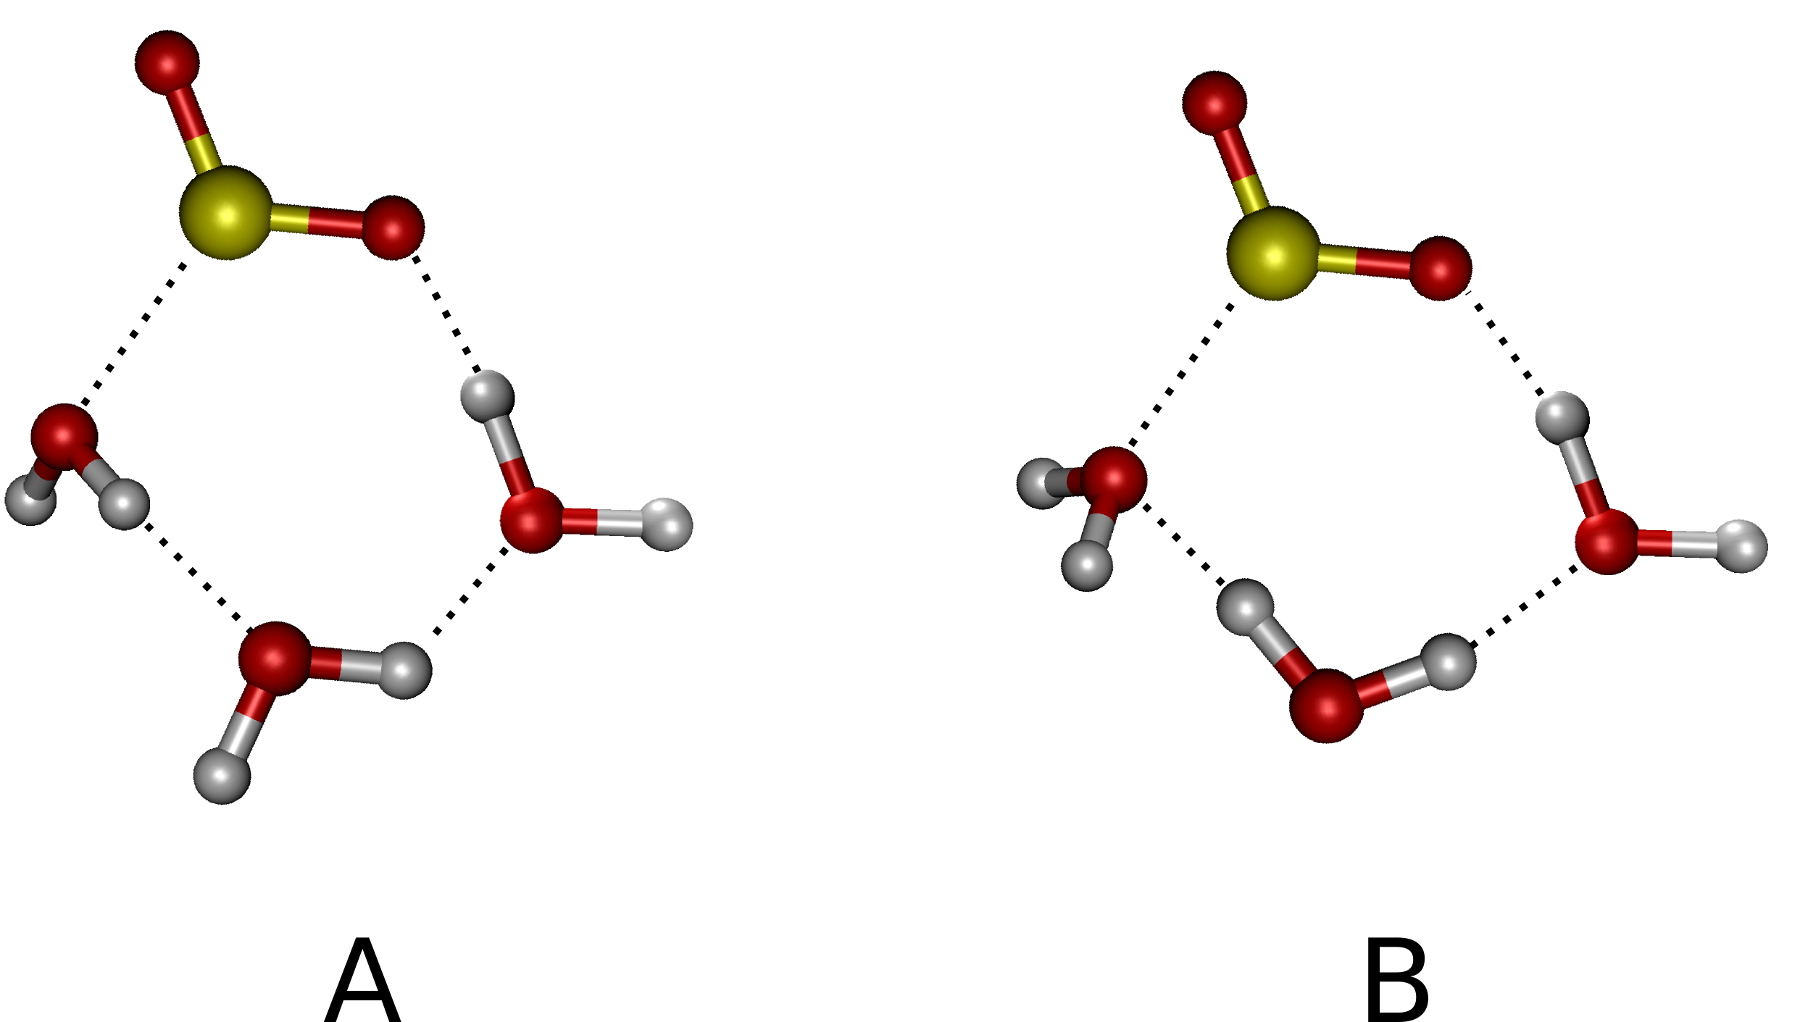
\includegraphics[scale=1.0]{images/cycles/triple-cycle-types-small.png}
		\caption{}
		\label{fig:type-3-varieties}
	\end{center}
\end{figure}
